\subsection*{Updated Data Flow Diagrams}

\subsubsection*{Level 0 DFD}

Here is our updated top level DFD:

\begin{center}
  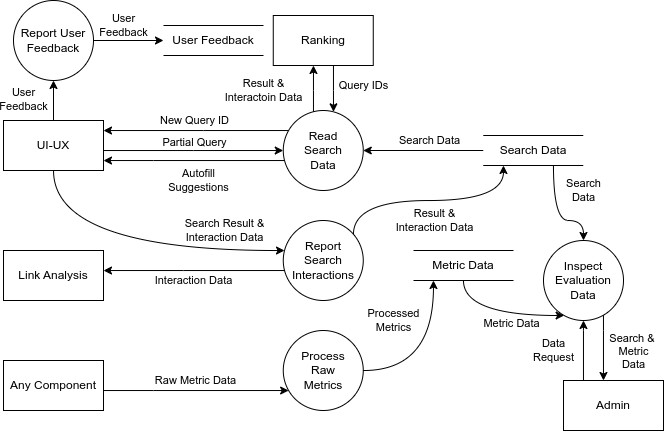
\includegraphics[scale=0.5]{DFDs/HighLevelDFD.drawio (1).png}
\end{center}
High Level Changes:
\begin{itemize}
  \item Ranking now asks for interaction data instead of us sending it to them on each query
  \item Added the Report User Feedback process for UI/UX
  \item Condensed read operations into one high level process
\end{itemize}

Report User Feedback is a simple operation, so no lower level DFDs are needed. The exact data received form UI/UX will be dumped to text files.

\newpage
\subsubsection*{Level 1 DFDs}

\textbf{Read Search Data}

\medskip

Both the Ranking and UI/UX components will need to read data from our database in one way or another. UI/UX will need autofill suggestions and unique query IDs. Neither of these are directly stored, the way the interaction data that Ranking needs is, but they will still rely on the database contents to do this.

\begin{center}
  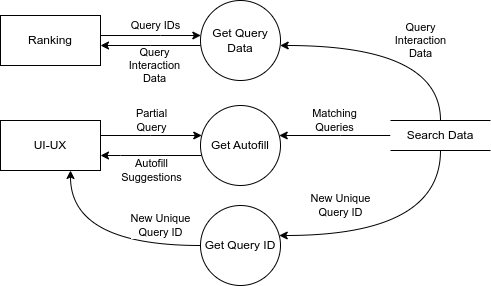
\includegraphics[scale=0.5]{DFDs/LowLevelDFDs-ReadSearchData.drawio.png}
\end{center}

\textbf{Report Search Interactions}

\medskip

After each query, the UI/UX team will send the user interaction data to us to be stored. Certain data will also be forwarded to Link Analysis for updating of the web-graph.

\begin{center}
  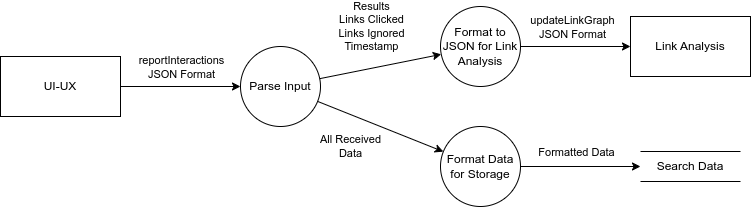
\includegraphics[scale=0.5]{DFDs/LowLevelDFDs-ReportSearchResults.drawio (2).png}
\end{center}

\textbf{Process Raw Metrics}

\medskip

All components will be sending metrics data periodically. This will be in a variety of formats, but will be aggregated together for storage in the Metric Data Database.

\begin{center}
  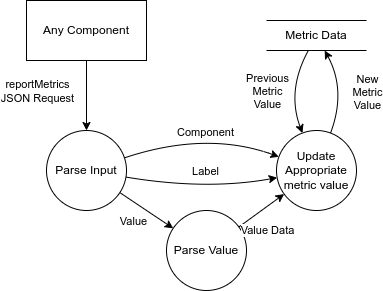
\includegraphics[scale=0.5]{DFDs/LowLevelDFDs-ReportMetric.drawio (1).png}
\end{center}

\newpage
\textbf{Inspect Evaluation Data}

\medskip

The system administrator will have the opportunity to interact with our component through a command line interface to inspect the logged search history as well as the performance metrics. 

\begin{center}
  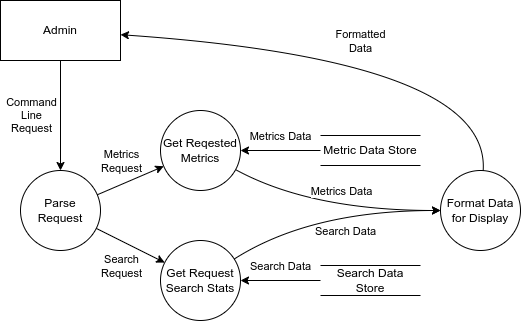
\includegraphics[scale=0.5]{DFDs/LowLevelDFDs-AdminView.drawio (1).png}
\end{center}

\subsubsection*{Level 2 DFD}

\textbf{Get Autofill}

\medskip

The other level 1 processes are relatively trivial, however autofill deserves a further expansion. We will attempt to correct typos, and search for similar queries (with and without typos). They will then be ranked and sent back to UI/UX.

\begin{center}
  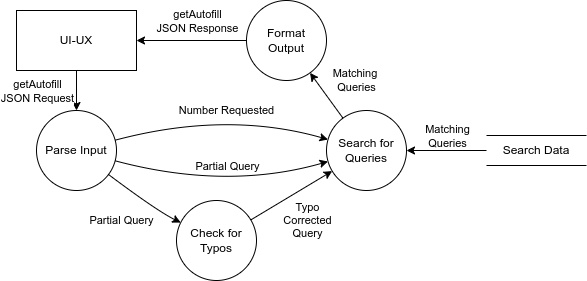
\includegraphics[scale=0.5]{DFDs/LowLevelDFDs-GetAutofill.drawio (2).png}
\end{center}

\newpage
\subsection*{Functional Decomposition Diagram}

This is our FDD:
\begin{center}
  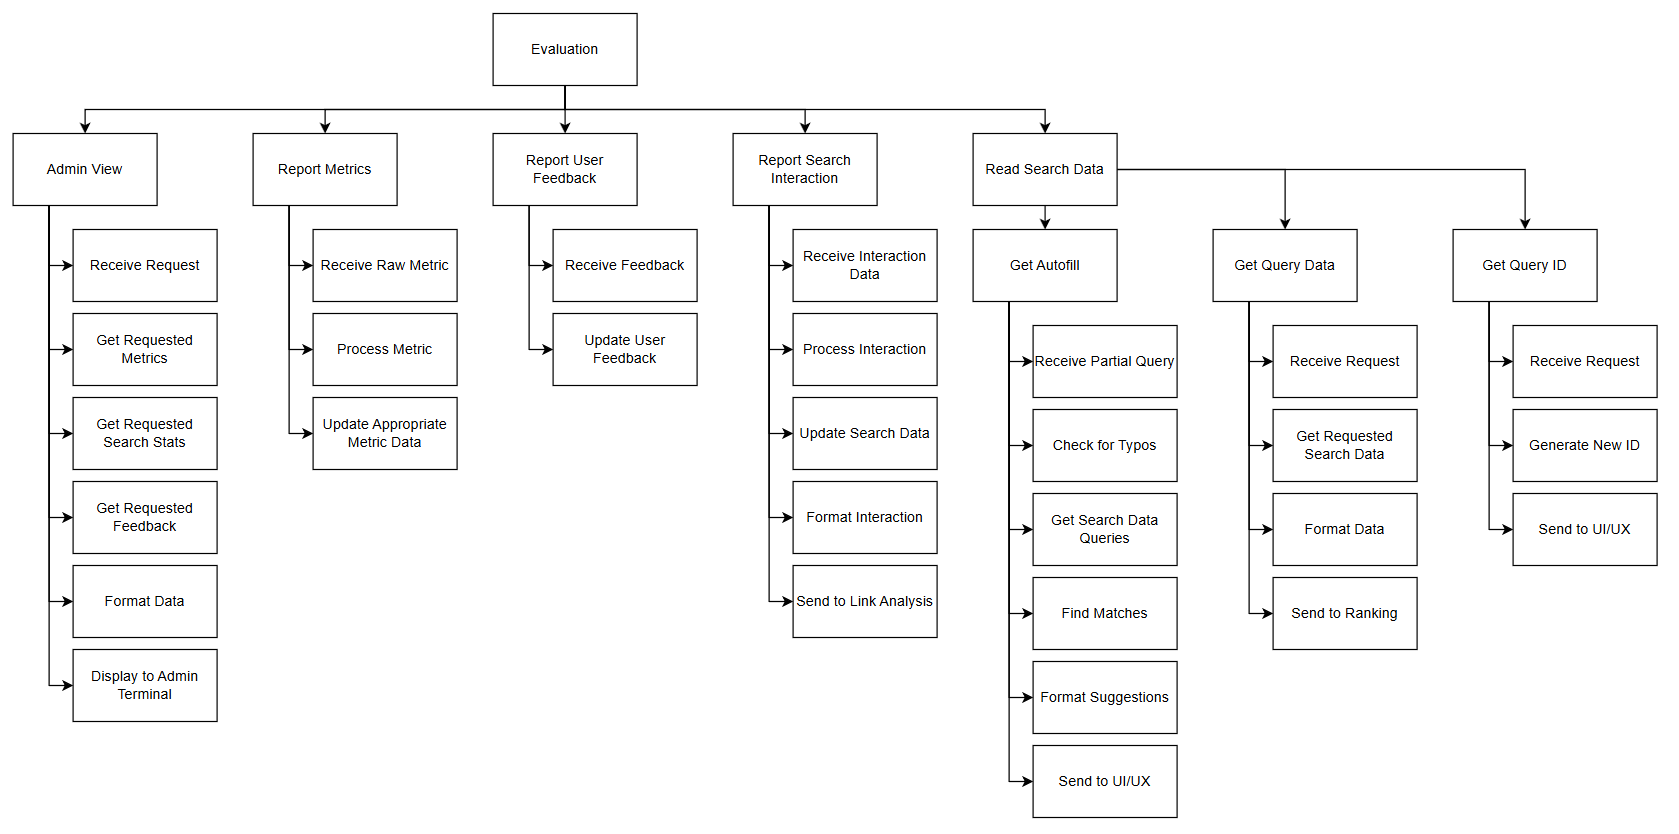
\includegraphics[width=\textwidth]{FDD/FDD.png}
\end{center}

\subsection*{Architectural Divisions}

\subsubsection*{Outgoing Calls}

These are functions which we will call for other components to take action on.

\medskip

\textbf{Function:} \verb|updateLinkGraph():|

\smallskip

\textbf{Destination Component:} Link Analysis

\smallskip

\textbf{Data Format:} \begin{verbatim}
  {
    "updates": [
      {
        "results": [ <List of links shown to the user> ],
        "clicked": <index in the above list of the result the user clicked>
      },
      <More JSON objects with the above format>
    ]
  }
\end{verbatim}

\smallskip

\textbf{Side Effects:} The stored web-graph will be updated with this information. This is the responsibility of the Link Analysis team.

\newpage
\subsubsection*{Incoming Calls}
These are the functions which other components will call for us to take action on.

\medskip

\textbf{Function:} \verb|reportMetrics():|

\smallskip

\textbf{Origin Component:} Any Component (All components will be calling this)

\smallskip

\textbf{Data Format:} \begin{verbatim}
  {
    "metrics": [
      {
        "label": <Label for the metric>
        "value": <Value for the metric>
      },
      <More metrics in the above format>
    ]
  }
\end{verbatim}

\smallskip

\textbf{Side Effects:} The metrics data that is sent will be stored for later use / display by a system Administrator.

\bigskip

\textbf{Function:} \verb|getAutofill():|

\smallskip

\textbf{Origin Component:} UI/UX

\smallskip

\textbf{Receive Data Format:} \begin{verbatim}
  {
    "num_suggestions": <Number of suggestions requested>,
    "partial_query": <The query which will be autofilled>
  }
\end{verbatim}

\textbf{Response Data Format:} \begin{verbatim}
  {
    "suggestions": [ <A list of suggestions for the complete query> ]
  }
\end{verbatim}

\smallskip

\textbf{Side Effects:} The above response will be sent to the UI/UX teams. They are responsible for showing these suggestions to the user.

\bigskip

\textbf{Function:} \verb|reportSearchResults():|

\smallskip

\textbf{Origin Component:} UI/UX

\smallskip

\textbf{Receive Data Format:} \begin{verbatim}
  {
    "query_ID": <Unique identifier of the query>
    "raw_query": <The exact query the user entered>,
    "results": [ <A list of results shown to the user> ],
    "clicked": <Index of the result the user chose in the above list>,
    "query_timestamp": <A timestamp for the query>
  }
\end{verbatim}

\smallskip

\textbf{Side Effects:} Our component will store all of this data, and call \verb|updateLinkGraph()|to propagate this information to the the web-graph.

\newpage

\textbf{Function:} \verb|getQueryID():|

\smallskip

\textbf{Origin Component:} UI/UX

\smallskip

\textbf{Receive Data Format:} \begin{verbatim}
  {}
\end{verbatim}

\textbf{Response Data Format:} \begin{verbatim}
  {
    "query_ID": <Unique identifier of the query>
  }
\end{verbatim}

\smallskip

\textbf{Side Effects:} This query ID will never again be returned by \verb|getQueryID|

\bigskip

\textbf{Function:} \verb|getQueryData():|

\smallskip

\textbf{Origin Component:} Ranking

\smallskip

\textbf{Receive Data Format:} \begin{verbatim}
  {
    "query_IDs": [ <List of unique identifiers of queries> ]
  }
\end{verbatim}

\textbf{Response Data Format:} \begin{verbatim}
  {
    "queries": [
      {
        "query_ID": <Unique identifier of the query>,
        "results": [ <A list of results shown to the user> ],
        "clicked": <Index of the result the user chose in the above list>
      }, 
      <More queries in the above format>
    ]
  }
\end{verbatim}

\smallskip

\textbf{Side Effects:} None

\bigskip

\textbf{Function:} \verb|submitFeedback():|

\smallskip

\textbf{Origin Component:} Ranking

\smallskip

\textbf{Receive Data Format:} \begin{verbatim}
  {
    "label": <Some Label for the feedback>,
    "title": <Some title for the feedback>,
    "text": <Some text for the feedback>
  }
\end{verbatim}

\smallskip

\textbf{Side Effects:} The feedback is stored for admin viewing.

\newpage
\subsection*{Design Review}

\subsubsection*{Internal Design Review}

\textbf{Date:} November 18, 2024 \\
\textbf{Duration:} 7:00 PM - 8:00 PM \\
\textbf{Participants:} Justin Ottesen (Team Lead), Kenji Chevray, Jayak Patel, Nahuel Fernandez \\
\textbf{Component Reviewed:} Evaluation Component

\medskip

\textbf{Objectives:}
\begin{itemize}
  \item Talk through the entire design plan to confirm details and resolve ambiguities
  \item Prepare for design review the following day with Document Data Store
\end{itemize}
Notes were taken first on a Word document, then on comments in the GitHub repository. The full write-up of the design review was completed the following day. It is accessible \href{https://docs.google.com/document/d/1REwOedsmrtoQbACQpFj3Ti8JiCDlrIysBp8OR26vRdU/edit?tab=t.0}{here}. The GitHub pull request with comments is accessible \href{https://github.com/justinottesen/LSPT-Evaluation/pull/27/commits/00ec74d93f1943b2d434e28471a2d04adcd9872c#diff-b335630551682c19a781afebcf4d07bf978fb1f8ac04c6bf87428ed5106870f5}{here}.

\medskip

As a result of our design review, these aspects of our design will be either updated or remain as previously decided upon:
\begin{enumerate}
  \item Sockets - UDP sockets will continue to be used\footnote{After our design review with DDS, our plans changed. Will be using REST API}.
  \item All information will be sent and received in JSON format as before. Additionally we will require a wrapper around all incoming messages to give additional information\footnote{After our decision to use REST API, the wrapper is no longer needed. This information will be replaced with header data.}.
  \item No ACK messages will be sent for any received metrics; the potential losses are offset by the increased ease of use and speed. Future releases may re-implement ACK messages.
  \item In the JSON wrapper for metrics, all components will need to have unique names, even those that have the same functionality, UI/UX, Indexing, Ranking, Link Analysis.
  \item Query ID will be of the type: Unsigned Integer
  \item All results from reportSearchResults will be identified using URL
  \item All metrics in search history will be maintained as planned. We had considered removing some metrics, but with low cost of storing, we would rather have too much than too little data.
  \item We will limit the maximum number of Query IDs that can be called in getQueryData.
  \item If there are bottlenecks, order of importance is: QueryID, Autofill, Everything else.
  \item Discussion of complete list of metrics requested from each component. Some additions, removals, and changes.
\end{enumerate}
In preparation for our design review with Document Data Store we condensed all data and prepared a couple of questions for them to provide feedback on.

\newpage
\subsubsection*{Document Data Store Design Review}

\textbf{Date:} November 19, 2024 \\
\textbf{Duration:} 8:00 PM - 8:45 PM (Our review of their design was 8:45 PM - 9:30 PM)\\
\textbf{Participants:} \\
Evaluation Team: Justin Ottesen (Team Lead), Kenji Chevray, Jayak Patel, Nahuel Fernandez \\
Document Data Store Team: Ben, Kale, Jose, Chaitanya \\
\textbf{Component Reviewed:} Evaluation Component

\medskip

\textbf{Objectives:}
\begin{itemize}
  \item Talk through our entire design plan to confirm details and resolve ambiguities. 
\end{itemize}

Notes were taken first on a Word document, and further feedback was relayed over discord. The full write-up of the design review was completed the following day. It is accessible \href{https://docs.google.com/document/d/1REwOedsmrtoQbACQpFj3Ti8JiCDlrIysBp8OR26vRdU/edit?tab=t.0}{here}.

\medskip

As a result of our design review, these aspects of our design will be either updated or remain as previously decided upon:
\begin{enumerate}
  \item Sockets - Ben has knowledge beyond what any of us have, and suggested using REST API. For now we are unsure, and need to do further research. The following day, we decided to change our format to use REST API
  \item We discussed potential RAM and storage problems associated with using a small VM. At this point we will do what we can with the available resources as will DDS and we will hope that more will be allocated to us in the future
  \item MongoDB. Because DDS will already be running an instance of MongoDB, DDS suggested that we use MongoDB to store the metrics received from other components. This will be our updated database for storing our metrics. 
  \item We added additional metrics to be received from both DDS and other components
  \item The remainder of our design plans remained as they were decided on in the internal review the previous day.
\end{enumerate}
Upon the completion of our design review, DDS began their design review. It was during their design review that mentions of MongoDB and the REST API were suggested to us. We provided similar discussion and feedback to their design review, and at the conclusion, we(both DDS and Evaluation) discussed more about the SE as a whole and sent out pings to everyone in the server to provide clarification about the SE as a whole.
